\documentclass[12pt,twoside]{article}
\usepackage[dvipsnames]{xcolor}
\usepackage{tikz,graphicx,amsmath,amsfonts,amscd,amssymb,bm,cite,epsfig,epsf,url}
\usepackage[hang,flushmargin]{footmisc}
\usepackage[colorlinks=true,urlcolor=blue,citecolor=blue]{hyperref}
\usepackage{amsthm,multirow,wasysym,appendix}
\usepackage{array,subcaption} 
% \usepackage[small,bf]{caption}
\usepackage{bbm}
\usepackage{pgfplots}
\usetikzlibrary{spy}
\usepgfplotslibrary{external}
\usepgfplotslibrary{fillbetween}
\usetikzlibrary{arrows,automata}
\usepackage{thmtools}
\usepackage{blkarray} 
\usepackage{textcomp}
\usepackage[left=0.8in,right=1.0in,top=1.0in,bottom=1.0in]{geometry}


\usepackage{times}
\usepackage{amsfonts}
\usepackage{amsmath}
\usepackage{latexsym}
\usepackage{color}
\usepackage{graphics}
\usepackage{enumerate}
\usepackage{amstext}
\usepackage{blkarray}
\usepackage{url}
\usepackage{epsfig}
\usepackage{bm}
\usepackage{hyperref}
\hypersetup{
    colorlinks=true,
    linkcolor=blue,
    filecolor=magenta,      
    urlcolor=blue,
}
\usepackage{textcomp}
\usepackage[left=0.8in,right=1.0in,top=1.0in,bottom=1.0in]{geometry}
\usepackage{mathtools}
\usepackage{minted}



%% Probability operators and functions
%
% \def \P{\mathrm{P}}
\def \P{\mathrm{P}}
\def \E{\mathrm{E}}
\def \Var{\mathrm{Var}}
\let\var\Var
\def \Cov {\mathrm{Cov}} \let\cov\Cov
\def \MSE {\mathrm{MSE}} \let\mse\MSE
\def \sgn {\mathrm{sgn}}
\def \R {\mathbb{R}}
\def \C {\mathbb{C}}
\def \N {\mathbb{N}}
\def \Z {\mathbb{Z}}
\def \cV {\mathcal{V}}
\def \cS {\mathcal{S}}
\DeclareMathOperator*{\argmin}{arg\,min}
\DeclareMathOperator*{\argmax}{arg\,max}
\newcommand{\red}[1]{\textcolor{red}{#1}}
\newcommand{\blue}[1]{\textcolor{blue}{#1}}
\newcommand{\green}[1]{\textcolor{ForestGreen}{ #1}}
\newcommand{\fuchsia}[1]{\textcolor{RoyalPurple}{ #1}}

%
%% Probability distributions
%
%\def \Bern    {\mathrm{Bern}}
%\def \Binom   {\mathrm{Binom}}
%\def \Exp     {\mathrm{Exp}}
%\def \Geom    {\mathrm{Geom}}
%\def \Norm    {\mathcal{N}}
%\def \Poisson {\mathrm{Poisson}}
%\def \Unif    {\mathrm {U}}
%
\newcommand{\bdb}[1]{\textcolor{red}{#1}}

\newcommand{\ml}[1]{\mathcal{ #1 } }
\newcommand{\wh}[1]{\widehat{ #1 } }
\newcommand{\wt}[1]{\widetilde{ #1 } }
\newcommand{\conj}[1]{\overline{ #1 } }
\newcommand{\rnd}[1]{\tilde{ #1 } }
\newcommand{\rv}[1]{ \rnd{ #1}  }
\newcommand{\rx}{\rnd{ x}  }
\newcommand{\ry}{\rnd{ y}  }
\newcommand{\ra}{\rnd{ a}  }
\newcommand{\rb}{\rnd{ b}  }
\newcommand{\rpc}{\widetilde{ pc}  }

\def \cnd {\, | \,}
\def \Id { I }
\def \J {\mathbf{1}\mathbf{1}^T}

\newcommand{\op}[1]{\operatorname{#1}}
\newcommand{\setdef}[2]{ := \keys{ #1 \; | \; #2 } }
\newcommand{\set}[2]{ \keys{ #1 \; | \; #2 } }
\newcommand{\sign}[1]{\op{sign}\left( #1 \right) }
\newcommand{\trace}[1]{\op{tr}\left( #1 \right) }
\newcommand{\tr}[1]{\op{tr}\left( #1 \right) }
\newcommand{\inv}[1]{\left( #1 \right)^{-1} }
\newcommand{\abs}[1]{\left| #1 \right|}
\newcommand{\sabs}[1]{| #1 |}
\newcommand{\keys}[1]{\left\{ #1 \right\}}
\newcommand{\sqbr}[1]{\left[ #1 \right]}
\newcommand{\sbrac}[1]{ ( #1 ) }
\newcommand{\brac}[1]{\left( #1 \right) }
\newcommand{\bbrac}[1]{\big( #1 \big) }
\newcommand{\Bbrac}[1]{\Big( #1 \Big)}
\newcommand{\BBbrac}[1]{\BIG( #1 \Big)}
\newcommand{\MAT}[1]{\begin{bmatrix} #1 \end{bmatrix}}
\newcommand{\sMAT}[1]{\left(\begin{smallmatrix} #1 \end{smallmatrix}\right)}
\newcommand{\sMATn}[1]{\begin{smallmatrix} #1 \end{smallmatrix}}
\newcommand{\PROD}[2]{\left \langle #1, #2\right \rangle}
\newcommand{\PRODs}[2]{\langle #1, #2 \rangle}
\newcommand{\der}[2]{\frac{\text{d}#2}{\text{d}#1}}
\newcommand{\pder}[2]{\frac{\partial#2}{\partial#1}}
\newcommand{\derTwo}[2]{\frac{\text{d}^2#2}{\text{d}#1^2}}
\newcommand{\ceil}[1]{\lceil #1 \rceil}
\newcommand{\Imag}[1]{\op{Im}\brac{ #1 }}
\newcommand{\Real}[1]{\op{Re}\brac{ #1 }}
\newcommand{\norm}[1]{\left|\left| #1 \right|\right| }
\newcommand{\norms}[1]{ \| #1 \|  }
\newcommand{\normProd}[1]{\left|\left| #1 \right|\right| _{\PROD{\cdot}{\cdot}} }
\newcommand{\normTwo}[1]{\left|\left| #1 \right|\right| _{2} }
\newcommand{\normTwos}[1]{ \| #1  \| _{2} }
\newcommand{\normZero}[1]{\left|\left| #1 \right|\right| _{0} }
\newcommand{\normTV}[1]{\left|\left| #1 \right|\right|  _{ \op{TV}  } }% _{\op{c} \ell_1} }
\newcommand{\normOne}[1]{\left|\left| #1 \right|\right| _{1} }
\newcommand{\normOnes}[1]{\| #1 \| _{1} }
\newcommand{\normOneTwo}[1]{\left|\left| #1 \right|\right| _{1,2} }
\newcommand{\normF}[1]{\left|\left| #1 \right|\right| _{\op{F}} }
\newcommand{\normLTwo}[1]{\left|\left| #1 \right|\right| _{\ml{L}_2} }
\newcommand{\normNuc}[1]{\left|\left| #1 \right|\right| _{\ast} }
\newcommand{\normOp}[1]{\left|\left| #1 \right|\right|  }
\newcommand{\normInf}[1]{\left|\left| #1 \right|\right| _{\infty}  }
\newcommand{\proj}[1]{\mathcal{P}_{#1} \, }
\newcommand{\diff}[1]{ \, \text{d}#1 }
\newcommand{\vc}[1]{\boldsymbol{\vec{#1}}}
\newcommand{\rc}[1]{\boldsymbol{#1}}
\newcommand{\vx}{\vec{x}}
\newcommand{\vy}{\vec{y}}
\newcommand{\vz}{\vec{z}}
\newcommand{\vu}{\vec{u}}
\newcommand{\vv}{\vec{v}}
\newcommand{\vb}{\vec{\beta}}
\newcommand{\va}{\vec{\alpha}}
\newcommand{\vaa}{\vec{a}}
\newcommand{\vbb}{\vec{b}}
\newcommand{\vg}{\vec{g}}
\newcommand{\vw}{\vec{w}}
\newcommand{\vh}{\vec{h}}
\newcommand{\vnu}{\vec{\nu}}
\newcommand{\rvnu}{\vc{\nu}}

\newtheorem{theorem}{Theorem}[section]
% \declaretheorem[style=plain,qed=$\square$]{theorem}
\newtheorem{corollary}[theorem]{Corollary}
\newtheorem{definition}[theorem]{Definition}
\newtheorem{lemma}[theorem]{Lemma}
\newtheorem{remark}[theorem]{Remark}
\newtheorem{algorithm}[theorem]{Algorithm}

% \theoremstyle{definition}
%\newtheorem{example}[proof]{Example}
%\declaretheorem[style=definition,qed=$\triangle$,sibling=definition]{example}
%\declaretheorem[style=definition,qed=$\bigcirc$,sibling=definition]{application}

%
%% Typographic tweaks and miscellaneous
%\newcommand{\sfrac}[2]{\mbox{\small$\displaystyle\frac{#1}{#2}$}}
%\newcommand{\suchthat}{\kern0.1em{:}\kern0.3em}
%\newcommand{\qqquad}{\kern3em}
%\newcommand{\cond}{\,|\,}
%\def\Matlab{\textsc{Matlab}}
%\newcommand{\displayskip}[1]{\abovedisplayskip #1\belowdisplayskip #1}
%\newcommand{\term}[1]{\emph{#1}}
%\renewcommand{\implies}{\;\Rightarrow\;}

% My macros

\def\Kset{\mathbb{K}}
\def\Nset{\mathbb{N}}
\def\Qset{\mathbb{Q}}
\def\Rset{\mathbb{R}}
\def\Sset{\mathbb{S}}
\def\Zset{\mathbb{Z}}
\def\squareforqed{\hbox{\rlap{$\sqcap$}$\sqcup$}}
\def\qed{\ifmmode\squareforqed\else{\unskip\nobreak\hfil
\penalty50\hskip1em\null\nobreak\hfil\squareforqed
\parfillskip=0pt\finalhyphendemerits=0\endgraf}\fi}

%\DeclareMathOperator*{\E}{\rm E}
%\DeclareMathOperator*{\argmax}{\rm argmax}
%\DeclareMathOperator*{\argmin}{\rm argmin}
%\DeclareMathOperator{\sgn}{sign}
\DeclareMathOperator{\supp}{supp}
\DeclareMathOperator{\last}{last}
%\DeclareMathOperator{\sign}{\sgn}
\DeclareMathOperator{\diag}{diag}
\providecommand{\abs}[1]{\lvert#1\rvert}
\providecommand{\norm}[1]{\lVert#1\rVert}
\def\vcdim{\textnormal{VCdim}}
\DeclareMathOperator*{\B}{\textbf{B}}

%\DeclarePairedDelimiter\ceil{\lceil}{\rceil}
%\DeclarePairedDelimiter\floor{\lfloor}{\rfloor}

\newcommand{\cX}{{\mathcal X}}
\newcommand{\cY}{{\mathcal Y}}
\newcommand{\cA}{{\mathcal A}}
\newcommand{\ignore}[1]{}
\newcommand{\bi}{\begin{itemize}}
\newcommand{\ei}{\end{itemize}}
\newcommand{\be}{\begin{enumerate}}
\newcommand{\ee}{\end{enumerate}}
\newcommand{\bd}{\begin{description}}
\newcommand{\ed}{\end{description}}
\newcommand{\h}{\widehat}
\newcommand{\e}{\epsilon}
\newcommand{\mat}[1]{{\mathbf #1}}
%\newcommand{\R}{\mat{R}}
\newcommand{\0}{\mat{0}}
\newcommand{\M}{\mat{M}}

\newcommand{\D}{\mat{D}}
\renewcommand{\r}{\mat{r}}
\newcommand{\x}{\mat{x}}
\renewcommand{\u}{\mat{u}}
\renewcommand{\v}{\mat{v}}
\newcommand{\w}{\mat{w}}
\renewcommand{\H}{\text{0}}
\newcommand{\T}{\text{1}}
%\newcommand{\set}[1]{\{#1\}}
\newcommand{\xxi}{{\boldsymbol \xi}}
\newcommand{\ssigma}{{\boldsymbol \sigma}}
\newcommand{\Alpha}{{\boldsymbol \alpha}}
\newcommand{\tts}{\tt \small}
\newcommand{\hint}{\emph{hint}}
\newcommand{\matr}[1]{\bm{#1}}     % ISO complying version
\newcommand{\vect}[1]{\bm{#1}} % vectors

%\newcommand{\Var}{\mathrm{Var}}
%\newcommand{\Cov}{\mathrm{Cov}}

% New commands
\newcommand{\SP}{\mathbf{S}_{+}^n}
\newcommand{\Proj}{\mathcal{P}_{\mathcal{S}}}
\DeclarePairedDelimiterX{\inp}[2]{\langle}{\rangle}{#1, #2}
\newtheorem{proof}{Proof}


\begin{document}

\begin{center}
{\large{\textbf{Homework 11}} } \vspace{0.2cm}\\
Due May 10 at 11 pm
\end{center}
Yves Greatti - yg390\\

\begin{enumerate}

\item (Lasso and $\ell_0$)
The file \texttt{X.txt} contains a $50 \times 300$ matrix $X$,
  and the file \texttt{y.txt} contains the $50\times 1$ vector
  $y$.  Each line of each file represents a row of the corresponding
  matrix, and the values on each line are space-delimited.
  \begin{enumerate}
  \item Consider the lasso problem
    $$\min_{\beta} \frac{1}{2n}\|X\beta -y\|^2 + \lambda\|\beta\|_1$$
    where $\lambda>0$ is a parameter and $n=50$.  Construct a (semilogx) plot
    that draws a
    separate path for each coefficient value as a function
    of~$\lambda$.
    Include values of $\lambda$ between $0.01$ and $2$ (you can
    include more if you want),
    and make your values spaced evenly on the log axis (e.g.,
    \texttt{np.geomspace}).  You can solve the lasso problem using

    whatever code/library you want.\\
   	\begin{figure}[H]
		\centering
		\captionsetup{justification=centering}
		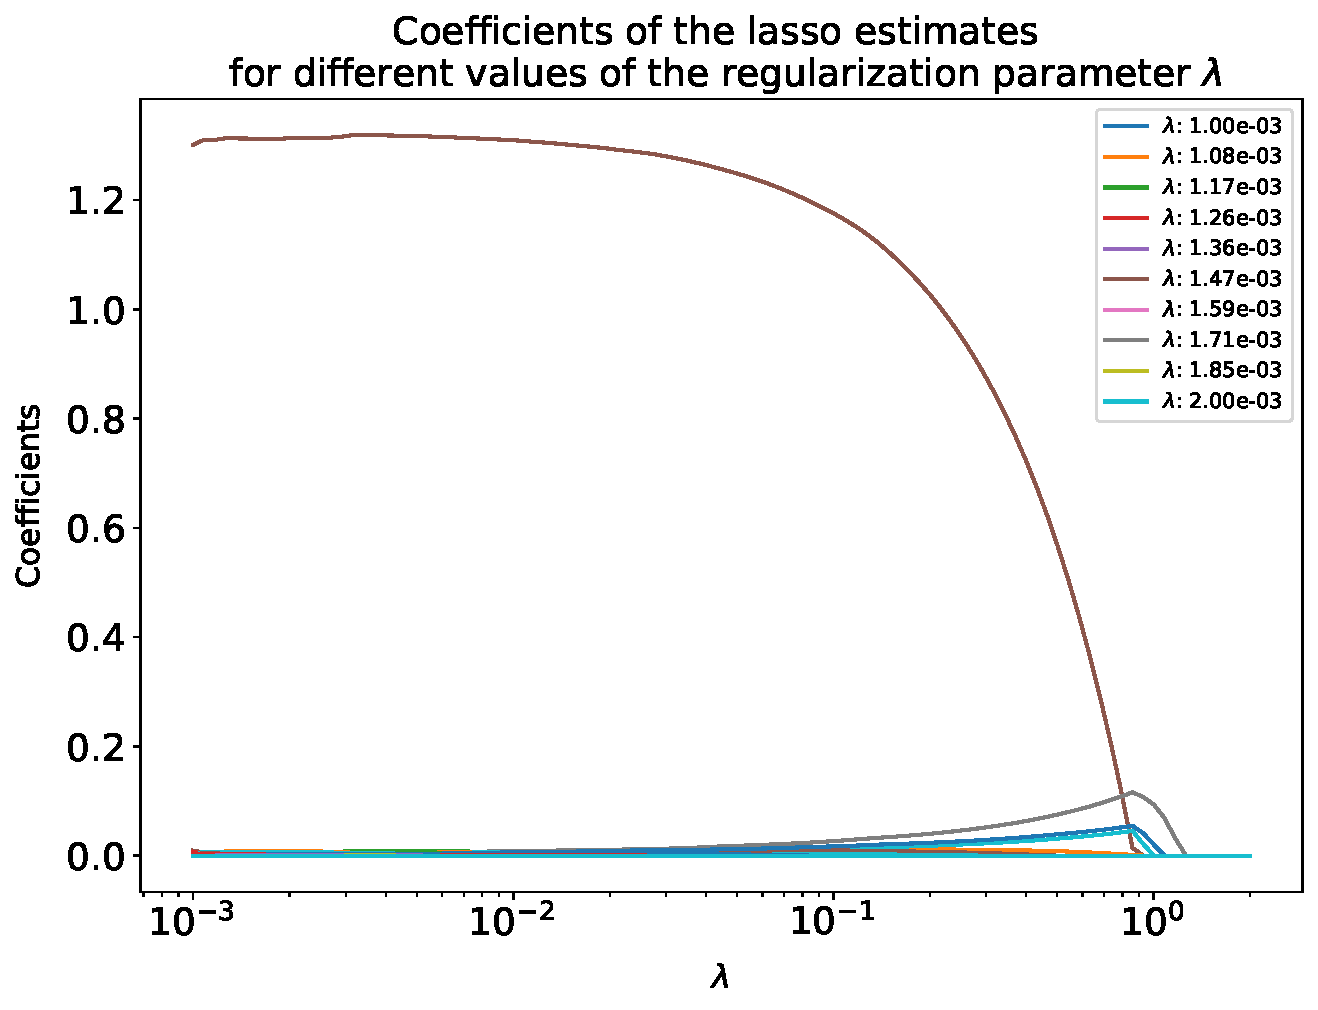
\includegraphics[width=200pt]{code/lasso_vs_lo/lasso.pdf}
	\end{figure}
 
  \item Determine the minimizer of
    $$\begin{array}{ll}
    \text{minimize} & \|\beta\|_0\\
    \text{subject to} & X\beta = y.
    \end{array}$$
    
    Assume that the minimizer has small $\ell_0$ norm, i.e $\ell_0 \leq 2$. Explain your strategy and justify that it finds the minimizer.  
    Report the nonzero coefficients of the minimizer, and
    their values.  Remember that two floating point values may be different for numerical reasons even if they represent the same value.\\
    
    We want to minimize the reconstruction loss $\argmin  \normTwo{X \beta - y}^2$ with  coefficient estimates $\beta$ having the minimum non-zeros elements.
    If we have to select only one column of $X$, we would choose the column which results in the largest projection of $y$ onto that column. 
    After selecting this column, we then solve the linear regression problem using that column with $y$ which gives us one coefficient estimate. We now compute the residual 
    between $y$ and that projection which we use as our new $y$. Reiterating the previous test, we find the second biggest "contributor" column by computing the inner product
    between the $residual$ and each of the columns of $X$. After identifying the new "best" column we now solve a linear regression problem, using the two selected columns so far, and $y$, which results in
    two new coefficient estimates, which is the sparse representation of $y$ using two columns of $X$. We keep iterating until we have the minimum number of nonzero coefficients $\beta$, the residual is less than a threshold, or we reach a maximum number of iterations.
    
 \begin{minted}{python} 
def orthogonal_mp(X:np.ndarray, 
	y:np.ndarray, 
	n_nonzero_coefs,  
	eps_min: np.float64 = 1e-3,
        iter_max: int = 1000):

    def stopping_condition(coef, n_nonzero_coefs):
        
        for i in range(len(coef)):
            if coef[i].shape[0] == n_nonzero_coefs:
                return True
        return False
        
    col_idx = list()
    coefs = list()
    residual = y   
    
    for _ in range(iter_max):
        i = np.abs(np.dot(X.T, residual)).argmax()
        if i not in col_idx:
            col_idx.append(i)
        
        coefi, _, _, _ = np.linalg.lstsq(X[:, col_idx], y)
        coefs.append(coefi)
        residual = y - np.dot(X[:,col_idx], coefi)
        
        if stopping_condition(coefs, n_nonzero_coefs):
            print(f"Found required number 
            of non-zero coefficients:{n_nonzero_coefs}")
            break
            
        #print(np.inner(residual, residual))
        if np.linalg.norm(residual) <= eps_min:
            print(f"Residual too small, less than {eps_min}")
            break
            
    return coefs, col_idx
\end{minted}
Applying this algorithm for  $\ell_0 \leq 2$, we found
    \begin{center}
    		\begin{tabular}{ | c | c |  }
    		\hline
			\text{column} 117 & \text{column} 239 \\
		\hline
			0.33641899 & 0.51962402 \\ 
		\hline
    	\end{tabular}
    \end{center}

    \item Will your strategy in (b) always find the optimal minimizer of any least-squares problem with $\ell_0$ regularization?
    No, the strategy in (b) will return a minimizer but not necessarily the optimal one. For example, due to numerical reasons if columns of the matrix $X$ are very coherent (inner product  between columns, very close to each other), then the algorithm might not select the right column (it has been shown that if mutual incoherence property condition is satisfied, defined  as $\max_{(i,j), i \neq j} \PROD{X[:,i}{X[:,j]} < \frac{1}{2K-1}$ then K-sparse signal can be recovered).
  \end{enumerate}
  
 \newpage
 \item (Proximal operator) The proximal operator of a function $f: \R^n \rightarrow \R$ is defined as
\begin{align}
\op{prox}_{f}\brac{y} := \arg \min_{x} f\brac{x}+ \frac{1}{2} \normTwo{x-y}^2.
\end{align}
  \begin{enumerate}
  \item Derive the proximal operator of the squared $\ell_2$ norm weighted by a constant $\alpha > 0$, i.e. $f(x)=\alpha \normTwo{x}^2$.

\begin{align*}
\op{prox}_{f}\brac{y} := \arg \min_{x}  \alpha \normTwo{x}^2 + \frac{1}{2} \normTwo{x-y}^2
\end{align*}

The two terms are quadratic, therefore differentiable, the gradient is 
$$
	\nabla_x \op{prox}_{f}\brac{y} = 2 \alpha x + (x-y)
$$
 Setting the gradient to zero, yields:
\begin{align*}
	2 \alpha x + (x-y)			&= 	0 \\
		x 					&= \frac{1} {1+2 \alpha} y \\
		\op{prox}_{f}\brac{y} 		&=	 \frac{1} {1+2 \alpha} y, \alpha > 0 \\
\end{align*}
 
  \item Prove that the proximal operator of the $\ell_1$ norm weighted by a constant $\alpha > 0$ is a soft-thresholding operator,
\begin{align}
\op{prox}_{\alpha \, \normOne{ \cdot }}\brac{ y } & = \ml{S}_{\alpha}\brac{y},
\end{align}
where 
\begin{align}
\ml{S}_{\alpha}\brac{y}[i] := 
\begin{cases}
y\,[i] - \op{sign}\brac{y\,[i]} \alpha  \qquad & \text{if $\abs{y\,[i]} \geq \alpha$}, \\
0 \quad & \text{otherwise}.
\end{cases}
\end{align}\\

$$
\op{prox}_{\alpha \, \normOne{ \cdot }}\brac{ y } = \alpha \|x\|_1 + \frac{1}{2} \normTwo{x-y}^2, \alpha > 0
$$
And we are looking for:
\begin{align*}
	0 \in \partial( \alpha \|x\|_1) + \nabla_x (\frac{1}{2} \normTwo{x-y}^2) \\
	0 \in \alpha \; \partial( \|x\|_1) + (x-y) \\
\end{align*}
We examine each component of $x$ and $y$ separately.
Assume first that $x[i] \neq 0$ then $ \partial( \|x\|_1) = \sign{x[i]}$, setting the subgradient to $0$, we have:
\begin{align*}
	x[i] - y[i] + \alpha \sign{x[i]}	&= 0 \\
	x[i]					&= y[i] - \alpha \sign{x[i]} \\
\end{align*}
Note that
\begin{align*}
	x[i] < 0, \sign{x[i]} = -1 &\rightarrow y[i] + \alpha < 0 \text{ ~ or }  y[i] < -\alpha < 0 \\
	x[i] > 0, \sign{x[i]} = 1 &\rightarrow y[i] - \alpha > 0 \text{ ~ or }  y[i] > \alpha > 0 \\
\end{align*}
thus in this case $\sign{x[i]} = \sign{y[i]}$ and the optimal point is $y[i] - \alpha \sign{y[i]}$.
In the case where $x[i]=0$, let $\gamma =  \partial(\|x\|_1), | \gamma | \le 1$ then it holds
\begin{align*}
	x[i] - y[i] + \alpha \gamma = 0 &\rightarrow y[i] - \alpha \gamma = 0 \\
							&	y[i] = \gamma \alpha \\
							& |y[i]| \le \alpha
\end{align*}
Putting all together, we get
\begin{align}
\op{prox}_{\alpha \, \normOne{ \cdot }}\brac{ y } = 
\begin{cases}
y\,[i] - \op{sign}\brac{y\,[i]} \alpha  \qquad & \text{if $\abs{y\,[i]} \geq \alpha$}, \\
0 \quad & \text{otherwise}.
\end{cases}
\end{align}

    \item Prove that if $X \in \R^{p \times n}$ has orthonormal rows ($p \leq n$) and $y \in \R^{n}$, then for any function $f$
\begin{align}
\arg \min_{\beta} \frac{1}{2} \normTwo{ y - X^T\beta }^2 + f(\beta) = \arg \min_{\beta} \frac{1}{2} \normTwo{ Xy - \beta }^2 + f(\beta).
\end{align}
The two expressions for the same function $f$ differs on the first term, so we want to show that
$$
\arg \min_{\beta} \normTwo{ y - X^T\beta }^2  =  \arg \min_{\beta} \normTwo{ Xy - \beta }^2
$$
$X$ having orthonormal rows: $X X^T = I$, and
\begin{align*}
	\normTwo{ y - X^T\beta }^2  	&= (y^T -\beta^T X) (y - X^T\beta) \\
						  	&= y^T y - y^T X^T \beta - \beta^T X y + \beta^T X X^T \beta \\
						  	&=   y^T y - y^T X^T \beta - \beta^T X y +  \beta^T \beta \\
	 \normTwo{ Xy - \beta }^2 		&= (y^T X^T - \beta^T) (Xy - \beta) \\
	 						&= y^T X^T X y - y^T X^T \beta - \beta^T X y +  \beta^T \beta \\
	\arg \min_{\beta} \normTwo{ y - X^T\beta }^2 &= \arg \min_{\beta}  \normTwo{ Xy - \beta }^2 \text{ eliminating terms independant of } \beta\\
\end{align*}

\item Use the answers to the previous questions to compare the ridge-regression and lasso estimators for a regression problem where the features are orthonormal.
  \end{enumerate}
The use of $l_1$, $l_2$ norms gives rise to the problems, for $\lambda > 0$:

\begin{align*}
\frac{1}{2} \argmin_\beta \| y - X^T \beta\|_2^2 + \lambda \|\beta\|_2^2	& \text{~ Ridge regression} \\
\frac{1}{2} \argmin_\beta \| y - X^T \beta\|_2^2 + \lambda \|\beta\|_1	& \text{~ Lasso regression}
\end{align*} 
which is equivalent from part c) to
\begin{align*}
 \argmin_\beta  \lambda \|\beta\|_2^2 + \frac{1}{2} \| \beta - X y \|_2^2 	& \text{~ Ridge regression} \\
 \argmin_\beta   \lambda \|\beta\|_1+    \frac{1}{2} \| \beta - X y \|_2^2 	& \text{~ Lasso regression}
\end{align*} 
From part a) and b), the solutions of these two problems are the proximal operators:
\begin{align*}
	\beta_{\text{ridge}}	&= 	 \frac{1} {1+2 \lambda} X y \\
	\beta_{\text{lasso}}	&= 	  \ml{S}_{\lambda}\brac{X y}\\
\end{align*} 
We see that the lasso solution shows sparsity: when the component wise least-square coefficients, $X y$, are not small they are shrunken towards $0$ by $\lambda$, and set to $0$ when they are small.
In contrast the ridge regression estimates are never sparse, all scaled with a single factor inversely proportional to $\lambda$. When $\lambda$ is $0$, ridge and lasso estimates are the OLS estimates.
 
 \newpage
  \item (Proximal gradient method)   
 \begin{enumerate}
 \item The first-order approximation to a function $f:\R^{p}\rightarrow \R$ at $x \in \R^{p}$ equals
 \begin{align}
f\brac{x} + \nabla f\brac{x}^T\brac{y-x}. 
\end{align}
We want to minimize this first-order approximation locally. To this end we fix a real constant $\alpha >0$ and augment the approximation with an $\ell_2$-norm term that keeps us close to $x$,
 \begin{align}
f_{x}(y) :=f\brac{x} + \nabla f\brac{x}^T\brac{y-x} +  \frac{1}{2 \, \alpha }\normTwo{y-x}^2.
\end{align}
 Prove that the minimum of $f_{x}$ is the gradient descent update $x- \alpha \nabla f\brac{x}$.\\
 For $\alpha > 0$,
 \begin{align*}
 	\nabla f_{x}(y) &= \nabla f\brac{x} +   \frac{1}{\alpha } (y - x) \\
 \end{align*} 
 Setting the gradient to $0$ gives
 \begin{align*}
 	\alpha \nabla f\brac{x} + (y - x)  &= 0\\
	y &= x - \alpha \nabla f\brac{x} \\
 \end{align*} 
 
\item 
Inspired by the previous question, how would you modify gradient descent to minimize a function of the form
\begin{align}
h(x) = f_1(x) + f_2(x),
\end{align}
where $f_1$ is differentiable, and $f_2$ is nondifferentiable but has a proximal operator that is easy to compute?\\
At iteration $x^{(k)}$, we want to stay close to the gradient update for $f_1(x^{(k)})$ and minimize $f_2(x^{(k)})$

\begin{align*}
   x^{(k+1)}  	&=  \arg \min_{x}  f_2\brac{x^{(k)}} + f_1\brac{x^{(k)}} + \nabla f_1\brac{x^{(k)}}^T\brac{x-x^{(k)}} +  \frac{1}{2 \, \alpha } \normTwo{x-x^{(k)}}^2 \\
			&=   \arg \min_{x}  f_2\brac{x^{(k)}} + 2 \alpha  f_1\brac{x^{(k)}} + \bigg( 2 \alpha \nabla f_1\brac{x^{(k)}}^T\brac{x-x^{(k)}} + \normTwo{x-x^{(k)}}^2  \\
			&+  \normTwo{\alpha  \nabla f_1\brac{x^{(k)}}^T}^2 \bigg) -  \normTwo{\alpha  \nabla f_1\brac{x^{(k)}}^T}^2 \\
			&=  \arg \min_{x}  f_2\brac{x^{(k)}} + 2 \alpha  f_1\brac{x^{(k)}} +  \normTwo{\alpha  \nabla f_1\brac{x^{(k)}}^T +  (x-x^{(k)}) }^2 -  \normTwo{\alpha  \nabla f_1\brac{x^{(k)}}^T}^2 \\
			&=  \arg \min_{x}  f_2\brac{x^{(k)}} + f_1\brac{x^{(k)}} +  \frac{1}{2 \, \alpha }   \normTwo{\alpha  \nabla f_1\brac{x^{(k)}}^T +  (x-x^{(k)}) }^2 -  
			\frac{1}{2 \, \alpha }    \normTwo{\alpha  \nabla f_1\brac{x^{(k)}}^T}^2 \\
			&=   \arg \min_{x}  f_2\brac{x^{(k)}} +   \frac{1}{2 \, \alpha }   \normTwo{\alpha  \nabla f_1\brac{x^{(k)}}^T +  (x-x^{(k)}) }^2 \text{ ~ removing terms independant of } x\\
			&=   \arg \min_{x}  f_2\brac{x^{(k)}} +   \frac{1}{2 \, \alpha }   \normTwo{x - (x^{(k)} - \alpha  \nabla f_1\brac{x^{(k)}}^T )} \\
			 &= \op{prox}_{f_2}\brac{x^{(k)} - \alpha \nabla f_1\brac{x^{(k)}}} \\
\end{align*}

\item Show that a vector $x^{\ast}$ is a solution to
\begin{align}
 \op{minimize} \quad & f_1\brac{x} + f_2\brac{x},
\end{align}
where $f_1$ is differentiable, and $f_2$ is nondifferentiable, and both functions are convex, if and only if it is a fixed point of the iteration you proposed in the previous question for any $\alpha > 0$.\\
if $x^{\ast}$ minimizes $f_1\brac{x} + f_2\brac{x}$  then
\begin{align*}
	x^{\ast} &= \op{prox}_{f_2} (x^{(k)}  - \alpha \nabla f_1 (x^{(k)}) \\
	& \text{ since both functions are convex } \\
	& \Leftrightarrow 0 \in \partial_x \bigg( f_2\brac{x^{(k)}} + f_1\brac{x^{(k)}} + \nabla f_1\brac{x^{(k)}}^T\brac{x-x^{(k)}} +  \frac{1}{2 \, \alpha }\normTwo{x-x^{(k)}}^2 \bigg) \\
	& \Leftrightarrow \alpha  \nabla_x f_1\brac{x^{(k)}}^T + x - x^{(k)} = 0 \\
	& \Leftrightarrow  x^{\ast} =  x^{(k)}  - \alpha \nabla_x f_1\brac{x^{(k)}}^T  \\
\end{align*}

%$x^{\ast}$ minimizes $f_1\brac{x} + f_2\brac{x}$ if and only if $0 \in \nabla  f_1\brac{x^{\ast}} + \partial f_2\brac{x^{\ast}}$.
%\begin{align*}
% 	x^{\ast} &= \op{prox}_{f_2} (x^{\ast}  - \alpha \nabla f_1(x^{\ast}))  \\
% 	& \Leftrightarrow 0 \in \partial{f_2\brac{x^{\ast}}} +  (x^{\ast} - (x^{\ast}  - \alpha \nabla f_1(x^{\ast})) \\
%	& \Leftrightarrow 0 \in  \nabla  f_1\brac{x^{\ast}} + \partial f_2\brac{x^{\ast}} \\
%\end{align*}

  \end{enumerate}
  
  \newpage
  \item (Iterative shrinkage-thresholding algorithm)   
 \begin{enumerate}
 \item What is the proximal gradient update corresponding to the lasso problem defined below? Your answer will involve a hyperparameter which we will call as $\alpha$. 
 \begin{align*}
 \frac{1}{2} \normTwo{y - X\beta}^2 + \lambda |\beta|_1
 \end{align*}
 
 From 2.(b), we have established:
 \begin{align*}
\op{prox}_{\alpha \, \normOne{ \cdot }}\brac{ x } & = \ml{S}_{\alpha}\brac{x} \\
\ml{S}_{\alpha}\brac{x}[i] &=  \op{sign}{\brac{x\,[i]}} \max{ (|\brac{x\,[i]}| - \alpha , 0) } \\
\end{align*}


Combining it with 3.(b) gives for
 \begin{align*}
 	g(x) &= f(x) + \lambda |x|_1 \, f \text{~ being differentiable} \\
 x^{(k+1)} &= 	\op{prox}_{\alpha \lambda \, \normOne{ \cdot }}\brac{ x^{(k)}  - \alpha \nabla_x f\brac{x^{(k)}}^T } = \ml{S}_{\alpha \lambda}\brac{x^{(k)}  - \alpha \nabla_x f\brac{x^{(k)}}^T }
\end{align*}
Plugging it back leads to the proximal gradient update corresponding to the lasso problem 
$$
	 \beta^{(k+1)} =  \ml{S}_{\alpha \lambda} 	(\beta^{(k)} + \alpha X^T (y - X \beta^{(k)}))
$$

 \item How would you check whether you have reached an optimum? How would you modify this to take into account possible numerical inaccuracies?
 For each iteration we can compare the value of the objective function for the new estimates $\beta$ with the value obtained for the previous estimated coefficients and if the absolute difference is less
than a tolerance (very small  value) then we know we have  reached an optimum (we can also improve that logic and check that the difference did not decrease for the last $n$ iterations).
% If we did not move with the proximal value far enough from the previous objective value in the direction of the gradient then we stop iterating, using notations from question 3.c:
% $$
%  |\op{prox}_{f_2} (x^{(k)}  - \alpha \nabla f_1 (x^{(k)}) - \bigg( f_2\brac{x^{(k)}} + f_1\brac{x^{(k)}} + \nabla f_1\brac{x^{(k)}}^T\brac{x-x^{(k)}} +  \frac{1}{2 \, \alpha }\normTwo{x-x^{(k)}}^2 \bigg)| < \epsilon
 %$$
 
 \item Implement the method and apply it to the problem in \texttt{pgd\_lasso-question.ipynb}. You have to fill in blocks of code corresponds to the proximal gradient update step and termination condition. Report all the generated plots.\\
  
    	\begin{figure}[H]
		\centering
		\captionsetup{justification=centering}
		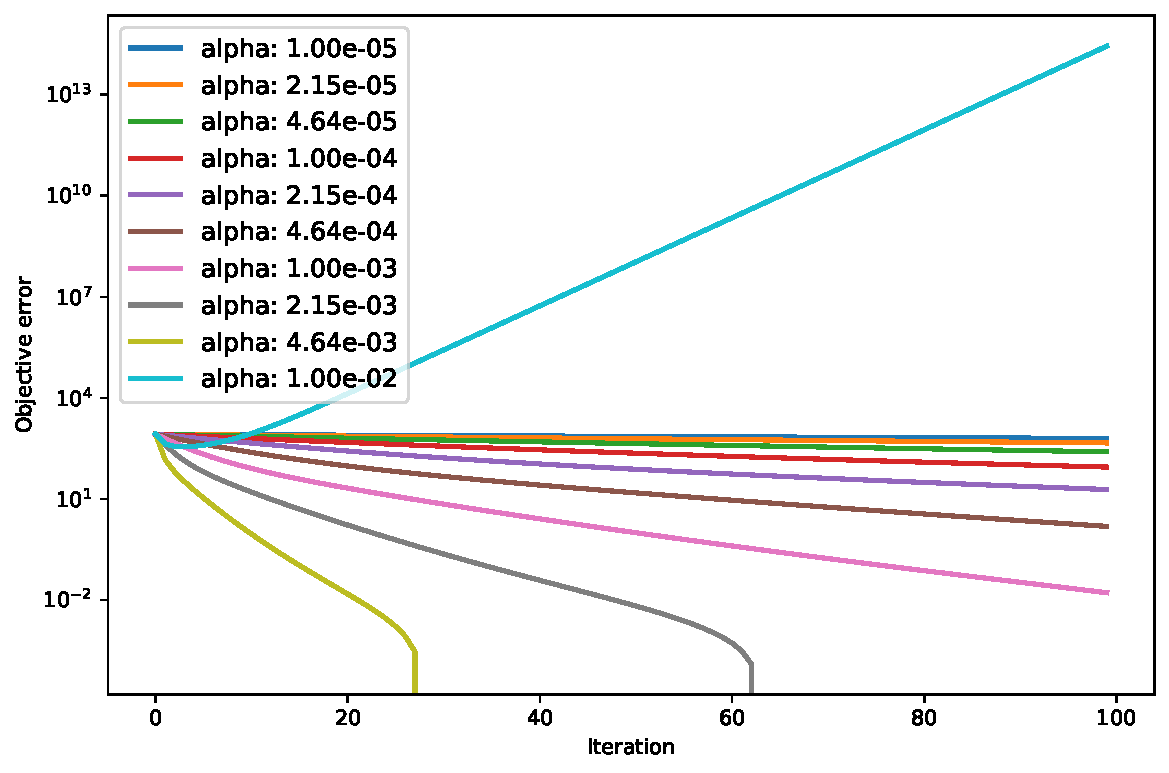
\includegraphics[width=200pt]{code/pgd/objective_error.pdf}
	\end{figure}

    	\begin{figure}[H]
		\centering
		\captionsetup{justification=centering}
		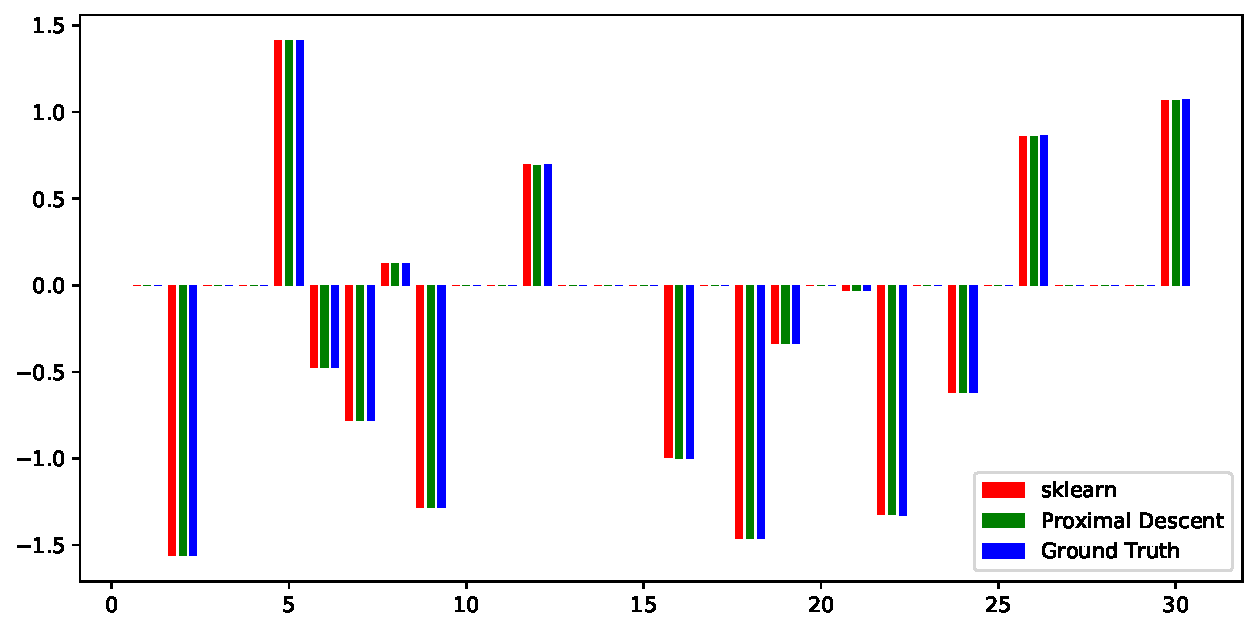
\includegraphics[width=200pt]{code/pgd/compare_models.pdf}
	\end{figure}

 \end{enumerate}
 

 \end{enumerate}
\end{document}
